%----------------------------------------------------------------------------
%----------------------------------------------------------------------------
%----------------------------------------------------------------------------
The distribution of molecular speeds in a gas is governed by Maxwell-Boltzmann statistics. This distribution impacts this study through the equation of motion (Equation \ref{final eom}) as a Doppler shift and through the ``geometric'' effects associated with linear molecular motion in the target region. The Doppler shift is proportional to the projection of the molecular velocity vector onto the laser beam wave front normal; the effects of the Doppler shift are described in Section \ref{doppler section}. The ``geometric'' effects are the temporal modulation of the excitation the molecule experiences by either leaving the excitation region before the pulse ends or entering the excitation region after the pulse has already started (or both). Additionally, the point in time at which the molecule emits its fluorescence photon may occur after the molecule leaves the region to which the receiver is sensitive.

The Maxwell-Boltzmann probability density function for molecular speeds is given by \cite{Serway:1990a}
%----------------------------------------------------------------------------
\begin{equation}
\rho(|v|)
=
\sqrt{\frac{2}{\pi}}
\left(\frac{m}{kT}\right)^{\frac{3}{2}}
v^2
\exp{\left(
-\frac{m v^2}{2 k T}
\right)}
\end{equation}
%----------------------------------------------------------------------------
where $k$ is the Boltzmann constant, T is the temperature (in K), $m$ is the molecular mass, and $v^2$ is the square of the molecular speed. See Figure \ref{Boltzmann-Maxwell} for a plot of this distribution.
%----------------------------------------------------------------------------
%----------------------------------------------------------------------------
%bb defines the bounding box for the pdf
%viewport defines the area of the pdf used
%in sidewaysfigure the last entry in bb moves the caption toward/away the pic
%in sidewaysfigure the second entry in bb moves the pic toward/away the caption
%----------------------------------------------------------------------------
\begin{figure}
\scalebox{0.8}[0.8]{
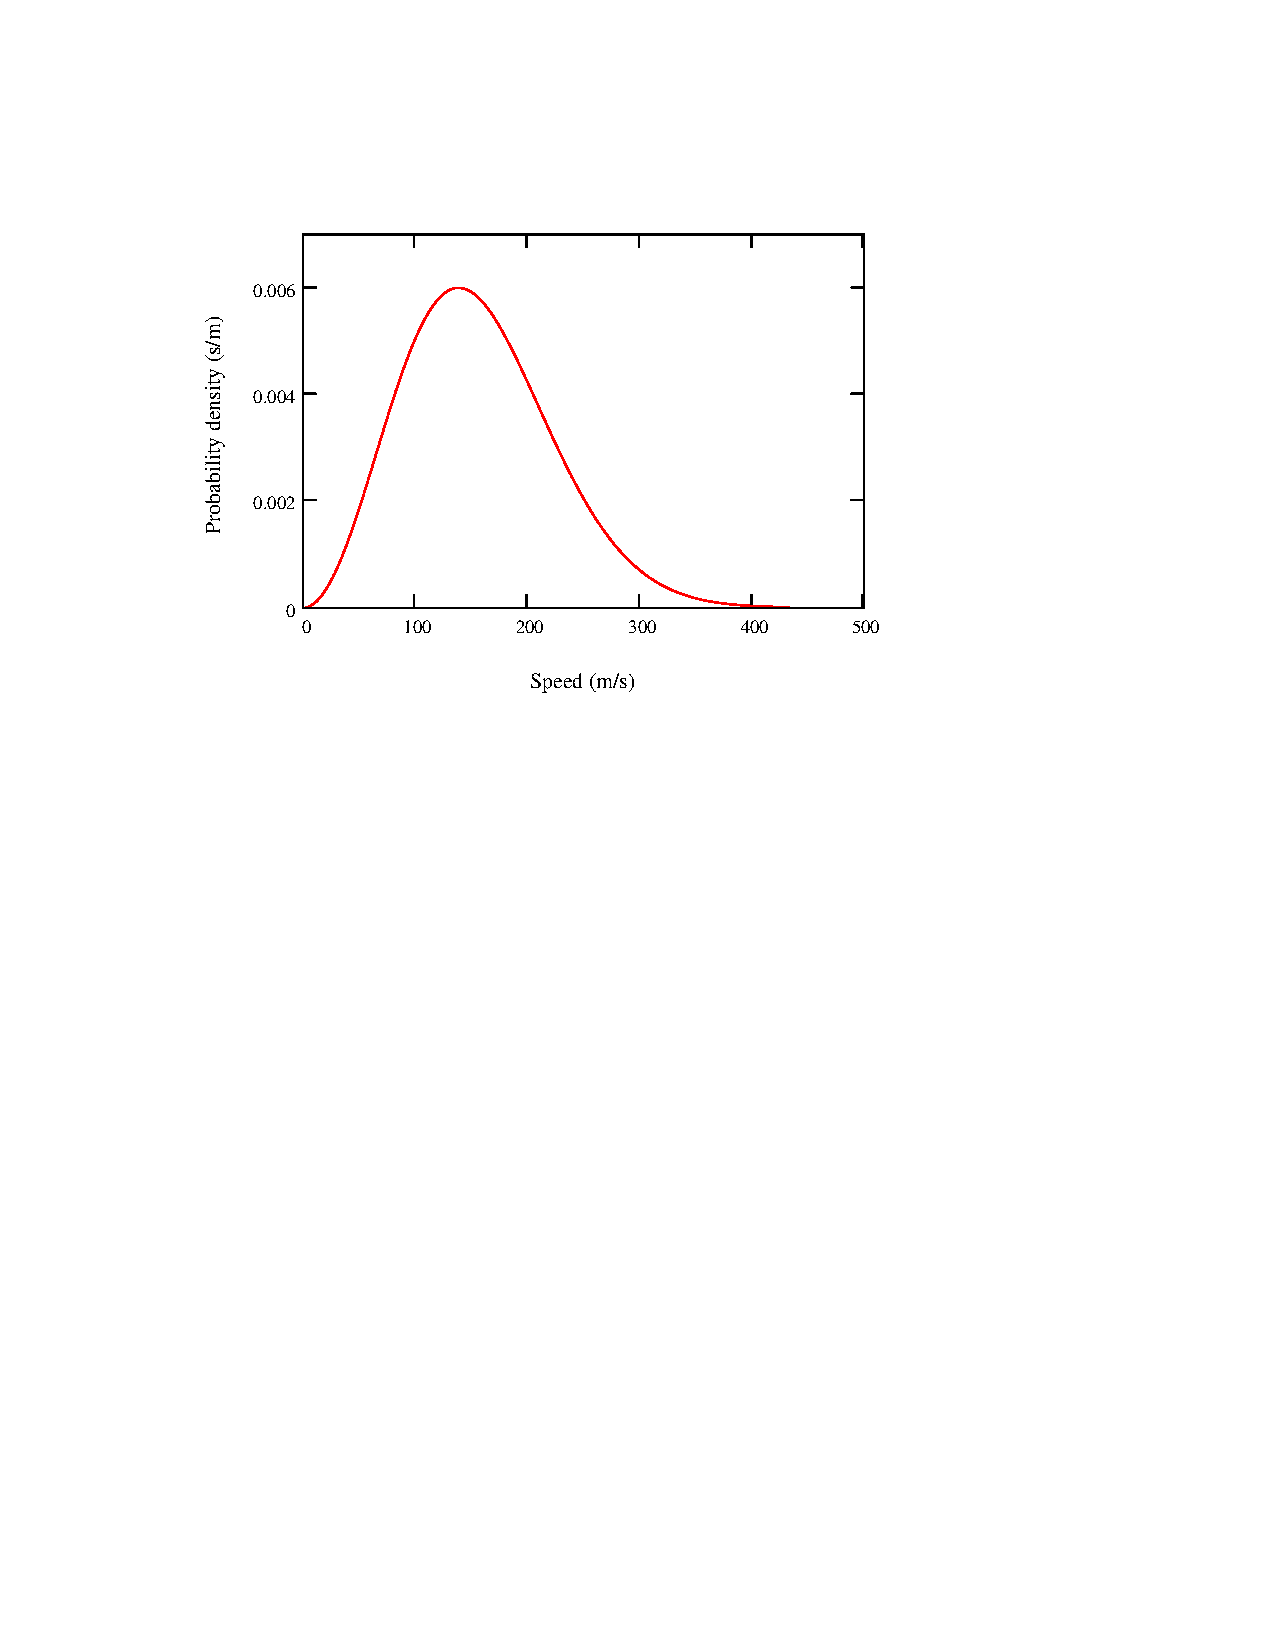
\includegraphics[bb=0 470 489 675]
{Boltzmann-Maxwell/Boltzmann-Maxwell.pdf}
}
\caption[Boltzmann-Maxwell distribution for molecular iodine]{Boltzmann--Maxwell distribution for molecular iodine. For this plot and associated simulations, $T=293$ K, $m = 2 \cross 127$ u (u $= 1.6605402\cross10^{-27}$ kg). The root mean square speed is 167 m/s, the average speed is 156 m/s, and the most probable speed is 139 m/s.}
\label{Boltzmann-Maxwell}
\end{figure}
%----------------------------------------------------------------------------

%----------------------------------------------------------------------------
%----------------------------------------------------------------------------
%----------------------------------------------------------------------------
